%!TEX root = ../../thesis.tex

\section{CDMA}
\label{sec:CDMA}

	This section will explain what CDMA is, alternatives and why it is needed.

	When transmitting data from a transmitter to a receiver over a channel, the entire channel is being used for this purpose.
	If one wants to have multiple transmitters transmitting over one channel, there is a problem. 
	The transmitters interfere with each other, this is called multiple access interference (MAI). 
	There are several ways to get around this problem: 

	\begin{itemize}
		\item TDM: Time Division Multiplexing. \\
				Each transmitter gets assigned a time slot, in which it and only it is allowed to transmit, hereby going around the MAI problem.
		\item FDM: Frequency Division Multiplexing. \\
				Each transmitters gets assigned a frequency band. Each transmitter is allowed to transmit the whole time, but only at the assigned frequencies.
		\item CDM: Code Division Multiplexing. \\
				Each transmitter gets assigned a code word. 
				The data first needs to be encoded using the code word and then the transmitter can send his message. 
				Each transmitter can transmit all the time using the entire frequency band. 
				These codes will determine how many transmitters can actually transmit with correct decoding results at the receiver end.
	\end{itemize}

	The distributed network of the VLC LEDs is inherently uncoordinated, since all the LEDs are basically only lights. 
	They have no receiver of any kind. 
	They can only implicitly transmit data by turning the load or the LED on or off.
	Because the LEDs cannot receive data, they cannot be assigned a time slot and therefor we cannot use a TDM scheme.

	An FDM scheme is also not applicable.
	This is because the LEDs do not have an explicit hardware transmitter that can modulate a signal.
	Instead the transmitting is implicitly done via turning the LED on and off.
	So only binary values of the current draw are sent as signals.

	This is where the CDM approach comes into play.
	This scheme allows the multiple LEDs to transmit at the same time.
	But the type of code used here is of importance.
	The code type determines the MAI and what the receiver is able to decode.

	\subsection{Performance metrics of a code}
	\label{subsec:performance-metrics}

		To determine which code is the best for this problem some measures are needed to be able to compare the codes.

		One such a measure is called the correlation.
		Correlation is a measure for determining how much sequence $X$ is similar to sequence $Y$ and can be found in \autoref{eq:correlation}.
		With $L$ being the length of the code and $\tau$ the time-shift.
		When sequence $X$ and $Y$ are the same sequence, we speak of the autocorrelation.
		When they are two different sequences, we speak of the cross-correlation. 

		\begin{equation}
			R(\tau)_{xy} = \displaystyle\sum_{i = 0} ^ {L - 1} x(i) \times y(i + \tau) {\text{  with $\tau = 0, 1, 2, \dotsc, L$}}
			\label{eq:correlation}
		\end{equation}

		The properties of an ideal code set should be, that the autocorrelation for each code in the set should be $0$ for each time-shift $\tau \neq 0$, at $\tau = 0$ the autocorrelation should be $L$.
		The ideal cross-correlation properties should $0$ for every time-shift $\tau$, so that no code interferes with any other code, hereby causing no MAI.

		Other metrics to be considered are the length of the code and how many codes there are in that code set.
		The code length is of importance because each bit a user will transmit must be encoded. 
		So the the message that will be transmitted via the channel will be the length of the code times the length of the data.
		If there are only a few codes in a code set then only a few number of users can transmit which does not scale well. 

	\subsection{Walsh-Hadamard Sequences}

		Walsh-Hadamard sequences are sequences which are created using a Hadamard matrix.
		Hadamard matrices are $n \times n$ matrices which are recursively generated.
		Starting with a $1 \times 1$ matrix: 
		$H_{1} = \begin{bmatrix} 1 \end{bmatrix}$, then 
		$H_{2} = \begin{bmatrix} 1 & 1 \\ 1 & -1 \end{bmatrix}$.
		Or in general: $H_{2n} = \begin{bmatrix} H_n & H_n \\ H_n & -H_n \end{bmatrix}$ \cite{714616}.
		The matrix can also be filled with binary values: zero and one. In that case the general matrix will be: 
		$H_{2n} = \begin{bmatrix} H_n & H_n \\ H_n & \overline{H_n} \end{bmatrix}$

		The Hadamard matrix has the property that every row in the matrix is orthogonal to every other row.
		Hadamard matrices exist for every power of $2$, so the code length is also a power of $2$.
		So for $\tau = 0$, the cross-correlation is $0$, but when $\tau \neq 0$ not all the rows are orthogonal anymore.
		\cite{1182447} proved that an Hadamard matrix of size $2^P$ could be divided into $P + 1$ subsets of rows, where one code could be selected giving $P + 1$ orthogonal codes for each time-shift $\tau$.
		These codes are called Cyclically Orthogonal Walsh Hadamard Codes (COWHC).

		All rows of the matrix have the property that the autocorrelation at $\tau = 0$ is equal to $L$.
		But when $\tau \neq 0$, undesirable behavior occurs as can be seen in \autoref{fig:autocorr-hadamard}.
		The autocorrelation function has several high peaks where only one is desired.
		This means that if a transmitter sends an encoded message with this code and the receiver does not know when in time the start of the message is, the receiver would get false positives for data.

		\begin{figure}
			\centering
			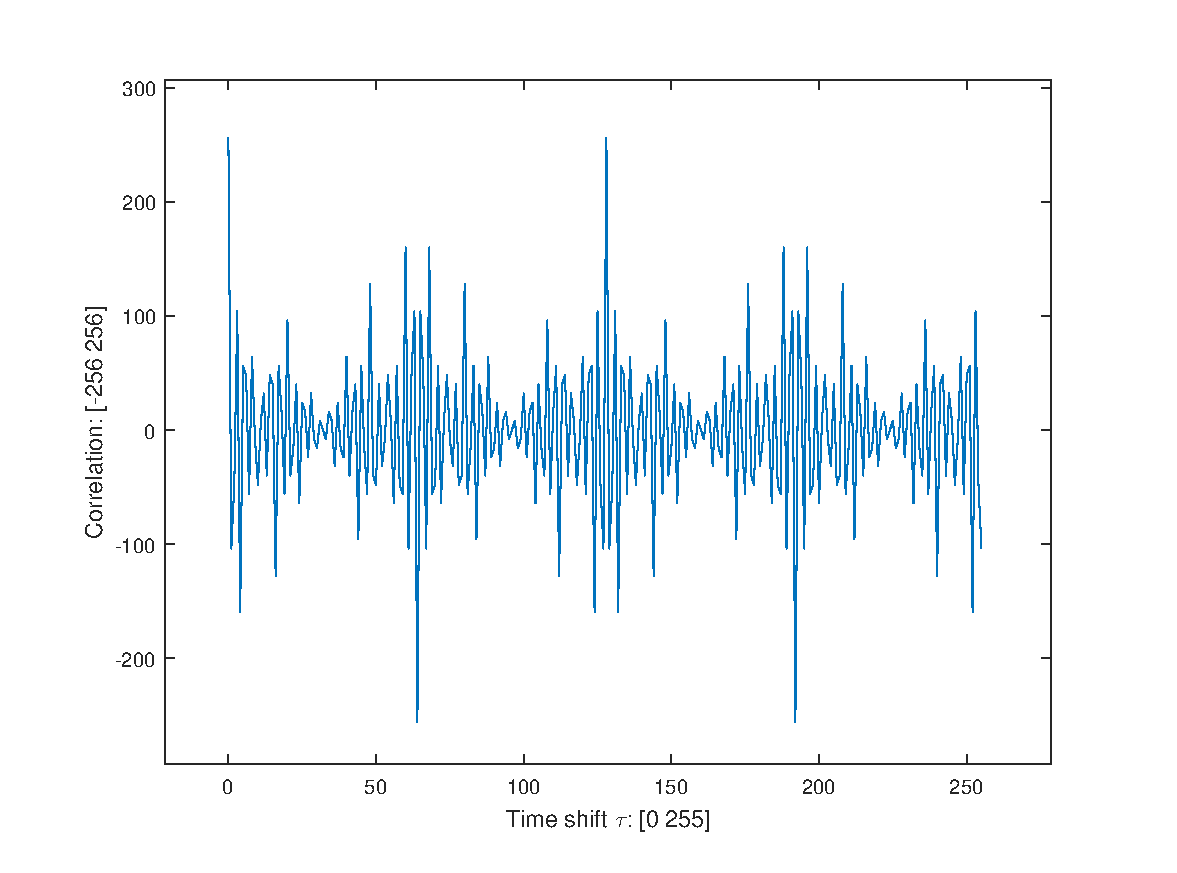
\includegraphics[width=\textwidth]{chapters/CDMA/autocorr-hadamard.eps}
			\caption{Autocorrelation of Hadamard code with index 120 of length 256.}
			\label{fig:autocorr-hadamard}
		\end{figure}

		So only a small subset of the codes have $0$ cross-correlation for every time-shift $\tau$ and the autocorrelation is far from what the ideal code set should have.


	\subsection{PN Sequences}

		PN sequences are sequences where the numbers looks like they are randomly generated but they are easily generated in software or hardware.
		The sequences have the following noise-like properties~\cite{mitra2008pseudo}:

		\begin{itemize}
			\item Balanced \\
					Any PN sequence of length $L = 2^n - 1$ contains exactly $2^{n-1}$ ones and $2^{n-1} - 1$ zeros.

			\item Runs \\
					A run is a subset of the sequence where all the consecutive numbers are the same.
					In any PN sequence, $1/2$ of the runs have length 1, $1/4$ have length 2, $1/8$ have length 3 and so on.

			\item Autocorrelation \\
					The autocorrelation function of a PN sequence will take on two values as can be seen in \autoref{eq:autocorr-pn} and \autoref{fig:autocorr-pn}.


		\end{itemize}

		\begin{equation}
			\label{eq:autocorr-pn}
			R(\tau) = 
				\begin{cases}
					L    & \quad \text{if } \tau = 0 \\
					-1   & \quad \text{if } \tau \neq 0 \\
				\end{cases}
		\end{equation}

		\begin{figure}
			\centering
			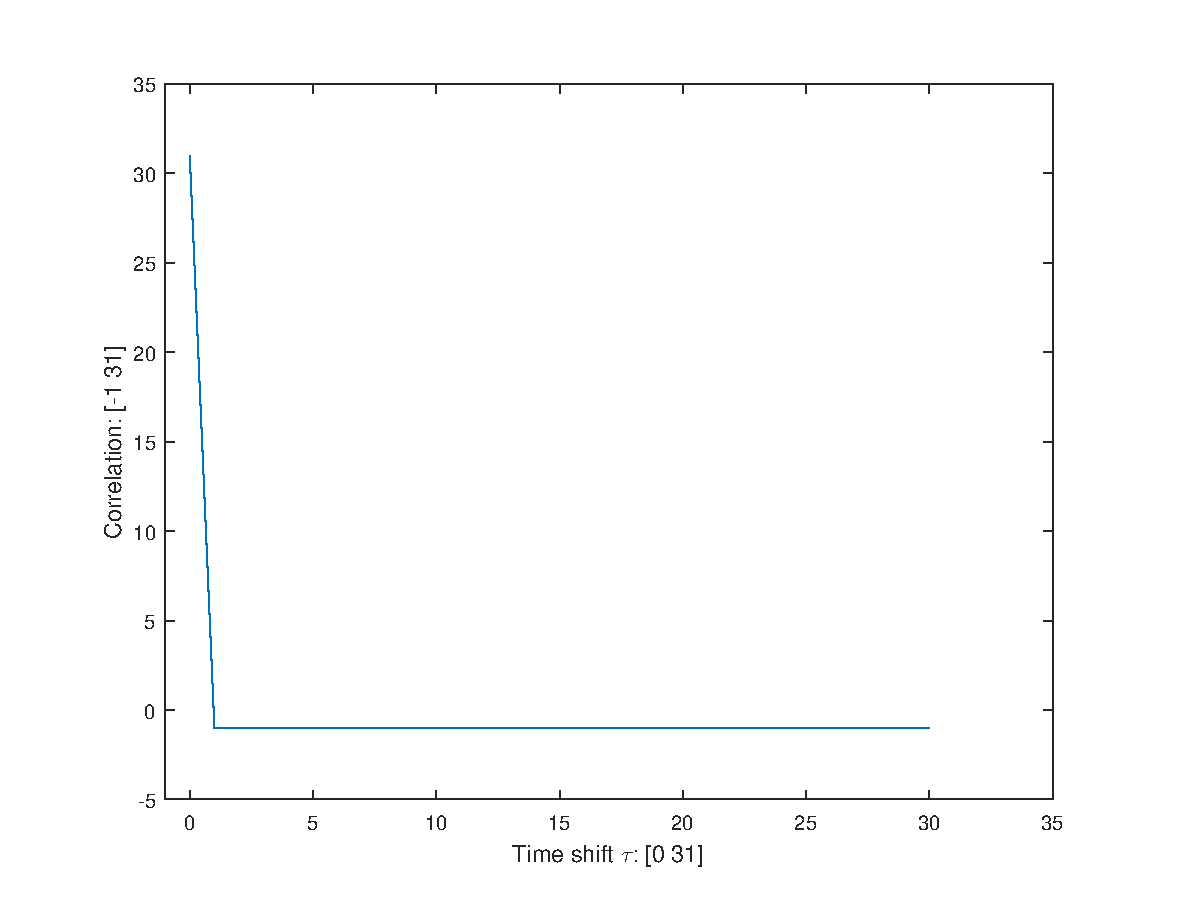
\includegraphics[width=\textwidth]{chapters/CDMA/autocorr-pn.eps}
			\caption{Autocorrelation of PN sequence of length 31.}
			\label{fig:autocorr-pn}
		\end{figure}

		PN sequences are generated using a linear feedback shift register (LFSR) \cite{Wang:1988:LFS:52007.52024}.
		\autoref{fig:lfsr} shows an $n$ length LFSR with some XOR gates attached to it.
		The LFSR is defined entirely by the feedback function, also called a characteristic polynomial.
		It determines the length and the type of sequence generated.
		The polynomial looks like \autoref{eq:lfsr-polynomial}.
		The LFSR in \autoref{fig:lfsr} contains $n$ shift registers and is initiated with a starting seed.
		This seed can be any vector apart from the all zero vector.
		The reason for this is because the XOR function with two zeros as input will output a zero, making the sequence that this LFSR outputs a sequence of all zeros.
		The output of the shift registers are multiplied with the coefficients of the characteristic polynomial ($C_{n-1}, C{n-2}, \dotsc, C_1, C_0$).
		The result output is then fed back into the first shift register, all the bits in the rest of the registers also shift one position and one output bit is created.
		With $n$ number of registers and the zero start vector excluded it takes $2^n - 1$ steps to output the entire sequence before it starts to repeat itself.


		\begin{figure}
			\centering
			\begin{tikzpicture}


				\node[block                  ] (last_register) {$s_{n-1}$};
				\node[block, right = 1cm of last_register] (second_last_register) {$s_{n-2}$};
				\draw[line] (last_register.east) -- (second_last_register.west) ;

				\node[block, right = 3cm of second_last_register] (second_register) {$s_{1}$};
				\node[block, right = 1cm of second_register] (mid_register) {$s_{0}$};
				\draw[line] (second_register.east) -- (mid_register.west) ;

				\draw[dashed, line] (second_last_register.east) -- (second_register.west) ;

				\node[coordinate, right = 2cm of mid_register] (output_point) {};
				\draw[line] (mid_register.east) -- (output_point.west) node [midway, above] {output};

				\node[XOR, scale=2, below = 2cm of second_register] (first_xor) {};
				\draw[line] (second_register.south) -- (first_xor.north) node [midway, right] {$C_1$};
				\draw[line] (mid_register.south) |- (first_xor.east) node [pos=0.21, right] {$C_0$};

				\node[coordinate, right = 1.5cm of second_last_register] (h) {};
				\node[XOR, scale=2, below = 2.5cm of h] (mid_xor) {};
				\draw[line] (first_xor.west) -- (mid_xor.east) ;
				\draw[dashed, line] (h.south) -- (mid_xor.north) ;

				\node[XOR, scale=2, below = 2cm of second_last_register] (second_last_xor) {};
				\node[XOR, scale=2, below = 2cm of last_register] (last_xor) {};

				\draw[line] (second_last_register.south) -- (second_last_xor.north) node [midway, right] {$C_{n-2}$};
				\draw[line] (mid_xor.west) -- (second_last_xor.east) ;
				
				\draw[line] (second_last_xor.west) -- (last_xor.east) ;
				\draw[line] (last_register.south) -- (last_xor.north) node [midway, right] {$C_{n-1}$};

				\node[coordinate, left = 1cm of last_register] (return_point) {};
				
				\draw[line] (last_xor.west) -| (return_point) -- (last_register.west) ;




			\end{tikzpicture}
			\caption{Linear feedback shifter register of length $n$, with XOR gates.}
			\label{fig:lfsr}
		\end{figure}

		\begin{equation}
			\label{eq:lfsr-polynomial}
			p(x) = x^n + C_{n-1} x^{n-1}  + C_{n-2} x^{n-2} + \dotsc + C_{2} x^{2}  + C_{1} x  + C_{0}
		\end{equation}


		Only certain polynomials will give a Maximal Length Sequence (MLS), or $m$-sequence.
		These sequences are per definition the largest codes that can be generated by a given shift register.

		% something about cross correlation....






		




